\documentclass[a4paper,11pt,oneside]{book}			
\usepackage[italian]{babel}			
\usepackage{lipsum}								
\usepackage{listings}							
\usepackage{url}								
\usepackage{graphicx}							
\usepackage{geometry}						
\usepackage[dvipsnames]{xcolor} 				
\usepackage[hidelinks]{hyperref}		
\usepackage{chngpage}

\usepackage{authblk}
\renewcommand\Authand{ e }

		
\geometry{a4paper,top=2cm,bottom=2cm,left=3cm,right=3cm,heightrounded,bindingoffset=5mm}
\raggedbottom									

\lstset{language=Java,						
	showspaces=false,
	showtabs=false,
	breaklines=true,
	showstringspaces=false,
	breakatwhitespace=true,
	commentstyle=\color{ForestGreen},
	keywordstyle=\color{blue},
	stringstyle=\color{red},
	identifierstyle=\color{Gray},
	basicstyle=\small\ttfamily
}


\begin{document}

\title{Appunti di Programmazione di Interfacce}

\author[1]{Simone Pepi}
\author[2]{Francesco Iannelli}
\affil[1] {Stesura appunti}
\affil[2]{Riscrittura in \LaTeX}
\date{a.a. 2019/2020 Prof. Mazzei}
\maketitle

\tableofcontents

\chapter{Introduzione}
\begin{flushleft}
	\textit{Che cos'è il design?}
\end{flushleft}
Il design è \textbf{la pianificazione o la specifica per la costruzione di un oggetto o sistema, o per l'implementazione di un'attività o un processo.} Si trova quindi agli antipodi della scomposizione del problema in sottopassaggi, cioè del pensiero computazionale.

Il design parte dalla base del problema e \textbf{identifica soluzioni per la causa del problema}.
Famosa è la frase: \textit{"Se vogliamo che agli utenti piaccia il nostro software, dobbiamo progettare le applicazioni come se fossero persone con cui ci piacerebbe uscire."}

Due delle caratteristiche più importanti di una buona progettazione sono \textbf{visibilità} e \textbf{comprensibilità}.

\begin{itemize}
	\item \textbf{Visibilità}: è possibile indovinare quali azioni sono possibili e come eseguirle?
	\item \textbf{Comprensibilità}: cosa significa tutto questo? Come va usato? Cosa significano tutti i vari comandi?
\end{itemize}

Nei dispositivi complessi la visibilità e la complessità richiedono l'uso di manuali d'istruzioni, ma questo lo accettiamo solo se il dispositivo è davvero complesso, ma dovrebbe essere del tutto superfluo per le cose semplici.

\section{XX Design}
Fin dai primi tempi dell'industria del design, la parola \textit{design} normalmente farebbe pensare a qualcosa riguardante la grafica. Il lettore potrebbe sentirsi confuso riguardo a tutte le sfumature di significato che assume questa parola nel mondo del lavoro.

Con l'evoluzione della tecnologia anche l'industria dei media si è evoluta, dalla stampa ai media sul web, mobile e software, così come l'industria del design.

I settori principali della progettazione che andremo a toccare sono: il \textbf{design industriale}, il \textbf{design dell'interazione} e il \textbf{design dell'esperienza utente}. Nessuno di essi è rigidamente definito ma è diverso il punto focale di ognuno:

\begin{itemize}
	\item \textbf{Design industriale}: creazione e sviluppo sia di concetti che di specifiche per ottimizzare la funzionalità, il valore e l'aspetto di prodotti e sistemi, con reciproco vantaggio per gli utenti e i produttori
	\item \textbf{Design dell'interazione}: l'attenzione è concentrata sul modo in cui le persone interagiscono con la tecnologia; lo scopo è migliorare la loro comprensione di ciò che si può fare, ciò che succede e ciò che è appena successo, basandosi su principi psicologici, tecnici ed estetici.
	      \pagebreak
	\item \textbf{Design dell'esperienza utente}: progettazione di prodotti, processi, servizi, eventi e ambienti, mirando soprattutto alla qualità e alla piacevolezza dell'esperienza complessiva.
\end{itemize}

Per rispondere chiaramente a qualsiasi domanda, dobbiamo innanzitutto illustrare le differenze tra \textbf{Graphic Desing}, \textbf{User Experience Design (UX Design)}, \textbf{User Interface Design (UI Design)}.

\section{UX Designer}
La \textbf{User Experience} è il modo in cui le persone si sentono \textbf{a livello psicologico} quando usano un prodotto. Ogni prodotto utilizzato da qualcuno ha una user experience: giornali, bottiglie di ketchup, poltrone reclinabili, maglioni di cardigan ecc...

Quindi l' \textbf{UX design} si occupa di come il prodotto viene recepito, la sensazione che dà, ed è molto diverso dal tradizionale design grafico.

I progettisti UX lavorano in modo da conferire al prodotto la migliore esperienza d'uso possibile, in modo da trasmettere, all'utente che ne farà uso, una sensazione di soddisfazione e non di frustrazione.
A tal fine vengono usati una varietà di strumenti tra i quali: analisi competitiva, interviste e sondaggi, il tutto per arrivare a costruire tipologie di \textit{personas} tra gli utenti del prodotto.

\textbf{Non si può progettare la User Experience, ma si può progettare per la User Experience}, ecco perché, per soddisfare appieno gli utenti che useranno il prodotto, è importante comprendere quali sono le loro necessità.

\section{UI Designer}
Dallo studio della UX si crea un abbozzo dell'interfaccia. Non si crea subito il wireframe finale, ma si parte da un analisi dei casi di studio. Esistono più tipi di casi di studio ed ognuno è specifico per delle personas, infatti, personas differenti hanno capacità differenti.

L'UI Design è un procedimento differente dal front-end developing: la materia progetta le guidelines che istruiscono il developer su come creare al meglio una UI.

Possiamo considerare la UI Design come \textbf{sotto area} della UX Desing.

\begin{figure}[!h]
	\centering
	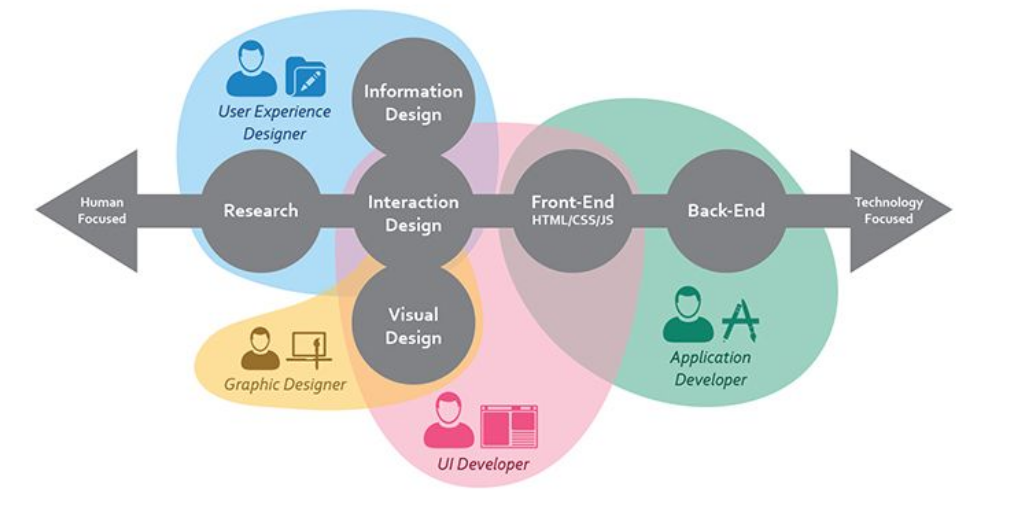
\includegraphics[scale = 0.4]{immagini/UX_and_UI.png}
	\caption{Le varie aree del design.}
\end{figure}


\chapter{User Interface}
Quando parliamo di \textbf{User Interface (UI)}, in italiano Interfaccia Utente, parliamo dello spazio di un sistema dove avviene l'interazione uomo-macchina: il monitor, il mouse, le casse audio e quant'altro.

L'obiettivo di questa interazione è far si che l'utente possa controllare e far funzionare la macchina in modo efficace, mentre la stessa macchina reagisce simultaneamente fornendo informazioni che aiutano il suo processo decisionale tramite \textbf{feedback}.

In generale, l'obiettivo dell' UI design è quello di produrre una UI che renda facile, efficiente e divertente l'uso di una macchina o di un programma, in modo da massimizzare la User Experience dell'utente finale.

Il termine \textbf{user-friendly} non può essere omesso in questa trattazione: tra un'app facile e piacevole da utilizzare e una solo facile da usare, l'utente medio preferirà sempre la prima.

Le interfacce sono strutturare in uno o più layer. L' \textbf{HID o Human Interface Device} è la periferica con cui l'utente interagisce con il sistema; come ad esempio mouse, monitor, gamepad, ecc...

Lo \textbf{HMI o Human Machine Interface} è un concetto che astrae dall' HID, con HMI, infatti, ci si riferisce allo strato che separa un essere umano che sta utilizzando una macchina dalla macchina stessa. Un device che implementa un HMI è un HID. Quando la macchina in questione è un computer, HMI diviene \textbf{HCI o Human Computer Interface}.

\section{Diversi tipi di interfacce}
Una persona umana possiede cinque differenti sensi che possono essere "mappati" in cinque categorie di interfacce possibili, più una categoria introdotta con l'introduzione di visori e giroscopi:
\begin{itemize}
	\item \textbf{tactile UI} (touch)
	\item \textbf{visual UI} (sight)
	\item \textbf{auditory UI} (sound)
	\item \textbf{olfactory UI} (smell)
	\item \textbf{equilibrial UI} (balance)
	\item \textbf{gustatory UI} (taste)
\end{itemize}
La composizione di più UI prende il nome di \textbf{CUI (Composite User Interface)}.
Le più comuni CUI sono le \textbf{GUI o Graphical User Interface}, le quali sono composte da interfacce grafiche e tattili. Se aggiungiamo anche il suono diventano \textbf{MUI (Multimedia User Interface)}.

\pagebreak

È bene sottolineare che \textbf{aggiungere più interfacce per poter interagire con una macchina utilizzando più sensi non è sempre una buona idea}. Giusto per fare un esempio, prendiamo in esame i video di Facebook: i video venivano riprodotti con l'audio attivo, ma gli ingegneri di Facebook si sono accorti che la maggioranza delle persone che visualizzavano i video, mutavano immediatamente il suono per varie ragioni (e.g. privacy o utilizzo di Facebook in momenti non opportuni), quindi hanno ben pensato di far partire la riproduzione automatica dei video con il suono mutato e introducendo i sottotitoli per le parti del video parlate. Questo oltre ad essere un ottimo esempio di MUI riprogettata in GUI è anche un esempio di tecnica ideata per le utenti disabili e riusata per poter far fruire il prodotto a quelle personas che lo utilizzano in momenti in cui non possono usufruire dell'audio.

\section{Categorizzare le CUI}
Le CUI possono essere categorizzare in tre diverse macrocategorie:

\begin{itemize}
	\item \textbf{Standard}: usano dispositivi standard come tastiere, mouse e monitor
	\item \textbf{Virtual}: \textbf{schermano} il mondo reale e creano un mondo virtuale. Tipicamente utilizzano dei caschi VR.
	\item \textbf{Augmented}: \textbf{non schermano} il mondo reale e erogano contenuti non completamente digitali che prendono forma nella realtà esterna che circonda l'utente, appunto espandendola.
\end{itemize}

Quando un'interfaccia utente interagisce con tutti i sensi umani viene chiamata \textbf{Qualia Interface}, secondo la \textbf{teoria Qualia}.

Le CUI possono essere anche \textbf{classificate per il numero di sensi} con cui esse interagiscono. Ad esempio, lo \textit{Smell-O-Vision} è una CUI standard 3S (3 sensi) con display, suono e odori. Se si aggiungesse un quarto senso diventerebbe un 4S, si pensi ad esempio alle poltrone dei famosi cinema 4D.

\begin{figure}[!h]
	\centering
	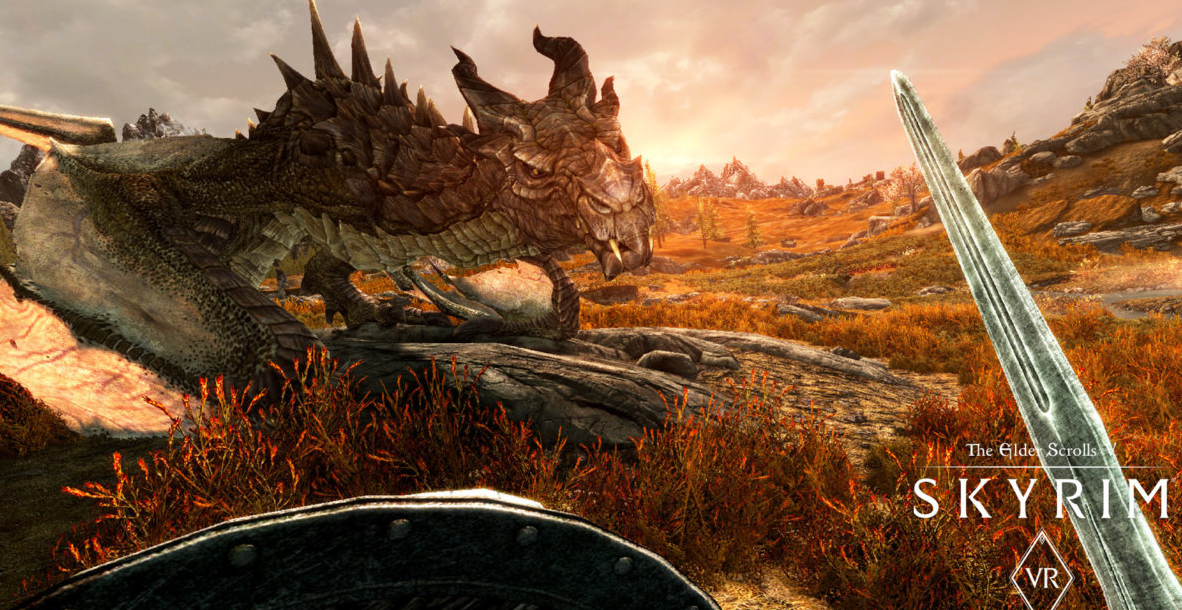
\includegraphics[scale = 0.15]{immagini/SkyrymVR.png}
	\caption{Virtual reality}
\end{figure}\begin{figure}[!h]
	\centering
	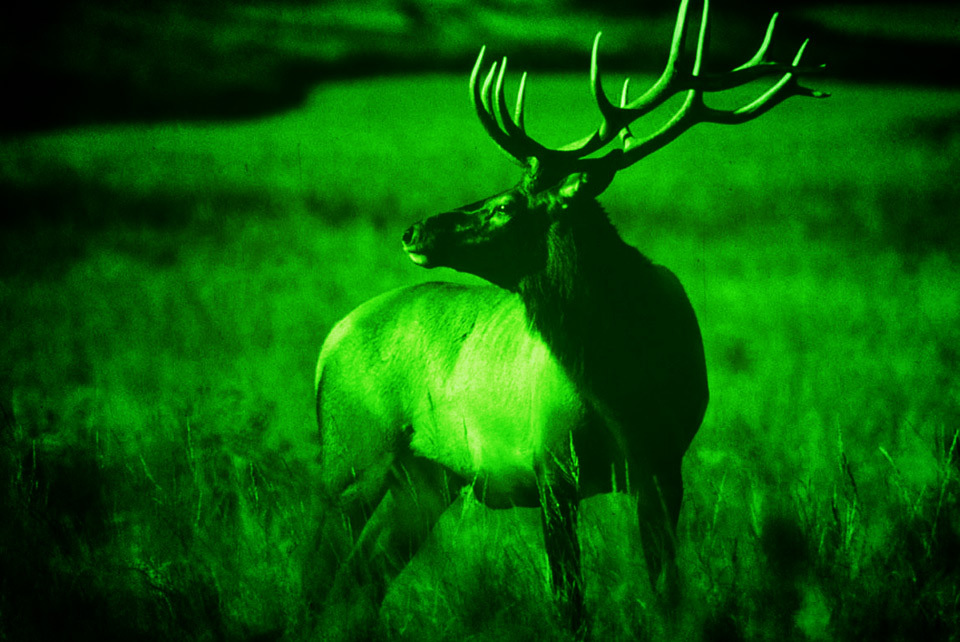
\includegraphics[scale = 0.15]{immagini/Night_vision.jpeg}
	\caption{Augmented reality.}
\end{figure}

\pagebreak


\chapter{Good and Bad Design}
Il buon design valido sempre e per tutti non esiste, poiché si fa design per la user experience di determinate personas. Però possiamo dare due caratteristiche importanti sui cui misurare un buon design:

\begin{itemize}
	\item \textbf{Discoverability}: è la capacità innata di un sistema di veicolare i possibili usi e di comunicare come si usa. Non è detto che una volta capito cosa si può fare si riesca a farlo. Per avere una buona discoverability si usa tipicamente la \textbf{visibilità}: un rubinetto con i pomelli bene in vista incrementa la discoverability. In un software tale lavoro è svolto dai pulsanti.
	\item \textbf{Understanding}: è la capacità del prodotto di farsi usare correttamente dall'utente.
\end{itemize}

\begin{figure}[!h]
	\centering
	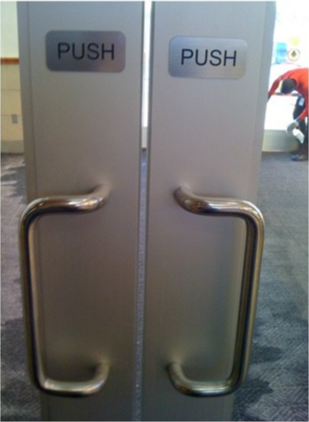
\includegraphics[scale=0.3]{immagini/vis.png}
	\caption{Discoverability and visibility.}
\end{figure}

\begin{figure}[!h]
	\centering
	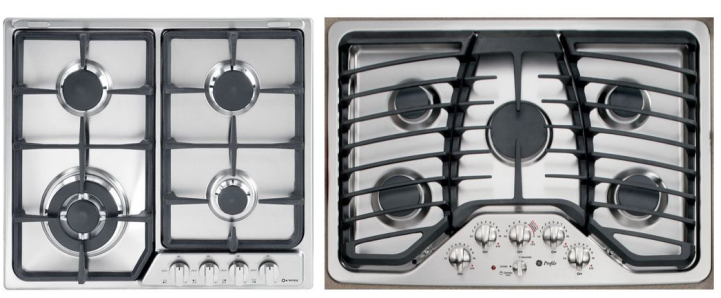
\includegraphics[scale=0.5]{immagini/Fornelli}
	\caption{Understanding.}
\end{figure}

\pagebreak

\section{Design of Useful Things}
\begin{flushleft}
	\textit{Quando le cose vanno bene, si dimenticano subito!}
\end{flushleft}
Questo perché nella psicologia umana le cose devono andare bene per definizione. Quando qualcosa va storto invece, l'amigdala crea un ricordo con un peso molto maggiore rispetto a un ricordo di una esperienza piacevole.

Il design deve quindi preoccuparsi di come funzionano le cose, come vengono controllate e della natura delle interazioni. Quando la progettazione è fatta bene, crea prodotti piacevoli e brillanti, quando è fatta mala, i prodotti sono inutilizzabili e ciò porta a una notevole frustrazione e irritazione.

Le macchine sono concepite, progettate e costruite da esseri umani. Al nostro confronto sono \textbf{assai limitate}: non conservano quella ricca storia di esperienze comuni che ci permettono di interagire grazie a un patrimonio collettivo di conoscenze.

Le macchine seguono di solito regole di comportamento rigide, piuttosto semplici. Se sbagliamo nel seguirle, anche di poco, la macchina fa quello che le diciamo, per quanto insensato e illogico sia. Noi esseri umani siamo creativi, dotati di immaginazione e pieni di buon senso, ovvero un abbondante patrimonio di sapere accumulato in anni di esperienza. Le macchine, però, ci obbligano a una grande precisione, cosa a cui non siamo avvezzi. Le macchine non hanno nè flessibilità nè buon senso e, spesso, gran parte delle regole seguite da una macchina è nota solo alla macchina stessa e ai suoi progettisti.

Quando non si eseguono queste sue regole segrete e bizzarre, e la macchina fa la \textbf{cosa sbagliata}, la colpa viene scaricata su chi la manovra, accusato di non capirla e di non seguirne i rigidi protocolli. Con gli oggetti di uso comune, il risultato è la frustrazione, con i dispositivi complessi o processi industriali e commerciali, le conseguenze possono essere incidenti anche mortali.

È tempo di \textbf{ribaltare la situazione}, di \textbf{accusare le macchine e la loro progettazione}. La colpa è delle macchine e di chi le ha progettate: sta a loro capire le persone, non a noi capire i loro dettami arbitrari e insensati.

Le ragioni delle carenze nell'interazione uomo-macchina sono numerose.

Alcune nascono dai limiti della tecnologia attuale, altre da limitazioni intenzionali dei progettisti, spesso per abbassare i costi di produzione. Ma la maggior parte dei problemi deriva dalla totale incomprensione dei principi di design necessari per un'efficiente interazione uomo-macchina. Perché questa deficienza? Perché la progettazione è opera per lo più di ingegneri esperti di ingegneria ma non di psicologia, quindi limitati nella comprensione delle persone.

\textit{"Siamo uomini anche noi"} pensano, \textit{"quindi siamo in grado di capire i nostri simili"}.

I tecnici fanno l'errore di pensare che sia sufficiente la spiegazione logica: \textit{"Basterebbe che leggessero le istruzioni e andrebbe tutto bene"}.

Gli ingegneri sono formati a un tipo di pensiero logico, di conseguenza finiscono per credere che tutti debbano pensare in quel modo e progettano le loro macchine di conseguenza.

\begin{center}
	\textbf{\LARGE Dobbiamo accettare il comportamento umano per quello che è, e non come vorremmo che fosse.}
\end{center}

\pagebreak


\chapter{Human Centered Design}
Le persone sono frustate dalla complessità degli oggetti quotidiani. Dalla complessità sempre maggiore del cruscotto dell'auto, alla crescente automazione della casa, con le sue reti interne. La proliferazione di sistemi complessi per il tempo libero e la comunicazione (e.g. video,audio,giochi elettronici) e le cucine sempre più tecnologiche; la vita di tutti i giorni sembra a volte una battaglia infinita contro la confusione, gli errori continui, la frustrazione, e un ciclo interminabile di aggiornamento e manutenzione degli apparecchi.

La soluzione è il \textbf{Design Antropocentrico} o \textbf{Human Centered Desing o HCD}, un'\textbf{impostazione che parte dai bisogni, dalle capacità e dai comportamenti umani, adattando la progettazione a quei bisogni, quelle capacità e quei comportamenti}. Lo HCD è un approccio di design specificamente orientato allo sviluppo di sistemi interattivi con l'obiettivo di produrre sistemi utili, altamente usabili e che si \textbf{focalizzano sull'utente}.

Il metodo è orientato all'efficienza ed all'efficacia , per aumentare la soddisfazione dell'utente ed evitare il più possibile gli effetti negativi.

\textbf{Prima l'utente, poi le features!} Lo HCD mette i bisogni, comportamenti e capacità umane prima di tutto, e progetta in funzione di esse.

Il problema principale delle UI è la comunicazione, in particolare la comunicazione dalla macchina verso la persona; \textbf{una buona interfaccia sa comunicare con l'utente}.

Progettare interfacce che funzionano fintanto che le cose vanno bene è relativamente facile, ma \textbf{la comunicazione è ancora più importante quando le cose non vanno bene}. È qui che i progettisti devono concentrare l'attenzione, sui casi in cui le cose vanno storte, non su quelli in cui le cose funzionano secondo i piani. Si focalizza l'attenzione soprattutto nel \textbf{comunicare ciò che è andato storto}: bisogna guidare l'utente frustato alla risoluzione del problema poiché, in caso di \textbf{risoluzione}, proverà una \textbf{sensazione positiva} di successo per aver capito cosa non funzionava e per aver risolto il problema. Ciò crea \textbf{empatia con il sistema}.

\textbf{Evitare quindi la frustrazione e aiutare a risolvere quando insorge un problema sono i concetti chiave dello HCD.}
Lo HCD è una filosofia di design che parte dalla \textbf{comprensione delle persone e dei bisogni che intende soddisfare}. Questa comprensione deriva dall'osservazione e dallo studio delle persone che spesso sono inconsapevoli dei loro veri bisogni e magari nemmeno delle difficoltà che incontreranno.

Per capire l'utente serve studio e osservazione della persona stessa. Non è sempre possibile tale osservazione, per cui versioni alfa e beta di un certo sistema non servono solo a fare debugging, ma servono anche per capire che cosa fa e come si comporta l'utente: diventa utile avere statistiche sull'utilizzo effettivo del sistema (e.g. quanti click su un determinato pulsante, quante volte una determinata procedura, ecc...)

\pagebreak

Ottenere \textbf{le specifiche dello HCD} è quindi una delle parti più difficili del design, al punto che il principio è quello \textbf{di evitare di specificare il più al lungo possibile} e procedere con ripetute approssimazioni: si esegue una specifica ad alto livello, se ne implementa una parte, si testa sull'utente finale e tramite il suo feedback, modifico la parte implementata e testo di nuovo. Quando si ritiene buono ciò che è stato implementato si congela e si passa ad implementare una nuova parte.

\begin{figure}[!h]
	\centering
	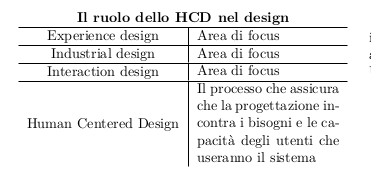
\includegraphics[scale=0.5]{immagini/HCD}
\end{figure}

Possiamo progettare per il design industriale, per l'interazione e per l'esperienza utente. Lo \textbf{HCD non è un'area di focus ma è un metodo}.

\section{Desing Thinking vs HCD}
Insieme al termine HCD, spesso si può vedere il termine \textbf{Design Thinking}. I due termini vengono da scuole di pensiero molto valide ma con visioni diverse.

Il Design Thinking segue il filone Stanford (dove è nato): è un \textbf{processo di desing} con cui progettare nuovi prodotti che verranno effettivamente adottati dalle persone. Come processo è più vicino alla \textbf{disruptive innovation} che all'antropocentricità.

Si suddivide in cinque fasi iterative:

\begin{itemize}
	\item \textbf{Empathize}: studiare il proprio pubblico, progettare il prodotto in modo che stabilisca un collegamento empatico con l'utente.
	\item \textbf{Define}: delineare meglio le domande chiave, cioè quali sono i bisogni a cui assolvere.
	\item \textbf{Ideate}: brainstorming, creare soluzioni.
	\item \textbf{Prototype}: costruire una o più idee.
	\item \textbf{Test}: testare òle idee e ricevere un feedback.
\end{itemize}

\begin{figure}
	\centering
	\includegraphics[scale=0.5]{"immagini/Fasi Design Thinking"}
	\includegraphics[scale=0.4]{"immagini/Design Thinking vs HCD"}
\end{figure}
Lo HCD è un mindset che viene sovrapposto al Design Thinking: identificato il modello di business, si può applicare lo HCD per assicurare che il prodotto soddisfi effettivamente le esigenze delle persone che lo andranno ad utilizzare.

\pagebreak

\chapter{Principi Fondamentali dell'Interazione}
I bravi designer producono esperienze piacevoli! Ai tecnici non piace molto la parola \textit{esperienza} poiché troppo soggettiva. Ma se si interrogasse un ingegnere sulla sua automobile preferita descriverà modello e finiture, la sensazione di potenza nell'accelerazione, la maneggevolezza del cambio e dello sterzo, ecc; queste sono esperienze.

L'esperienza è cruciale poiché determina la tonalità del ricordo che conserviamo delle interazioni con gli oggetti.

Quando la tecnologia si comporta in maniera inaspettata, proviamo confusione, frustrazione e rabbia: \textbf{emozioni negative}. Se invece comprendiamo il comportamento della tecnologia, abbiamo una sensazione di controllo, bravura e persino orgoglio: \textbf{emozioni positive}.

\textbf{Cognizione ed emozione sono profondamente legate}: se non mettiamo l'utente in un mood positivo farà più fatica ad apprendere l'interfaccia; più l'utente è arrabbiato e frustrato meno è predisposto a comprendere e riutilizzare il prodotto.

La \textbf{visibilità} o \textbf{discoverability} di un prodotto è il grado di facilità con cui un utente \textbf{scopre cosa fa, come funziona e che tipo di azione è possibile}. Tale visibilità è il risultato dell'applicazione di cinque concetti psicologici fondamentali: \textbf{affordance}, \textbf{significante}, \textbf{vincolo}, \textbf{mapping} e \textbf{feedback}. C'è anche un sesto principio, forse il più importante di tutti: \textbf{il modello concettuale del sistema}.Analizziamoli passo passo.

\section{Affordance}
Il termine affordance, letteralmente \textit{invito}, indica la relazione fra un oggetto fisico e una persona, cioè la relazione fra le proprietà dell'oggetto e la capacità dell'utente di determinare in che modo tale oggetto può essere usato.

\textit{Una sedia appare fatta apposta per sostenere qualcosa quindi "invita" alla seduta. La maggior parte delle sedie è abbastanza leggera da poter essere sollevata e spostata da una singola persona ("invita", "permette" al trasporto), ma qualcuna è così pesante da richiedere l'intervento di più persone. Se però un certo gruppo di individui non ha la forza di sollevare una sedia, per loro la sedia non presenta l'affordance "sollevamento e trasporto"}.

Una affordance \textbf{non è una proprietà ma è una relazione tra un oggetto e una persona}, dipende quindi dalle proprietà sia dell'oggetto che della persona.

Si può anche parlare di \textbf{anti-affordance} nel concetto di \textbf{prevenzione dell'interazione}. Un ottimo esempio sono gli spunzoni per evitare che piccioni o altri tipi di volatili si posino in un cornicione: prevengono l'affordance di sedersi che il cornicione ha verso i piccioni.
Le affordance e le anti-affordance \textbf{devono essere discoverable e perceivable}.

\pagebreak

Questo fatto non è scontato: il vetro, famoso per la sua relativa invisibilità, occulta l'anti-affordance di precludere il passaggio.

Se uno di questi inviti o impedimenti all'uso non è percepibile c'è bisogno di qualche mezzo per segnalarne la presenza: il significante.

\textbf{\underline{N.B.}} È assolutamente sbagliato dire "metto un affordance". Posso dire "metto un significante" ma solo se ho un'affordance.

\section{Significante}
I progettisti hanno dei problemi pratici: hanno bisogno di sapere come rendere comprensibili gli oggetti che creano. Lavorando sulla grafica degli schermi elettronici, dovevano trovare il modo di indicare quali parti potevano essere sfiorate, battute, scivolate in su o in giù o di lato, azioni che si potevano eseguire con le dite, con lo stilo o con il mouse.

Un significante è quindi \textbf{un modo per indicare dove effettuare un'azione}, dato un'affordance che determina quali azioni sono possibili.

\begin{figure}[!h]
	\centering
	\includegraphics[scale = 0.7]{"immagini/Affordance vs Signifier"}
\end{figure}
\begin{itemize}
	\item \textbf{Affordance}: cosa posso fare, quale azione posso compiere.
	\item \textbf{Signifier}: dove poso fare l'azione.
\end{itemize}
Molto spesso i significanti \textbf{sono indispensabili} poiché la maggior parte delle affordance sono invisibili. Per fare un esempio basti pensare alle porte scorrevoli: se i cardini non sono visibili, quando si vede la maniglia la prima azione che una persona tenta di fare è quella di spingere o tirare la porta, ma essa non si muoverà; è quindi necessario mettere un significante (e.g. un cartello o una scritta) che indica quale azione è necessaria per poter aprire la porta.

I significanti posso essere:
\begin{itemize}
	\item \textbf{Voluti o intenzionali}: come un'etichetta, una stringa, un'icona.
	\item \textbf{Accidentali o non intenzionali}: come ad e esempio un sentiero tracciato da persone che camminano attraverso un campo o delle persone in fila alla stazione.
\end{itemize}
Nel design \textbf{i significanti sono molto più importanti delle affordance}, perchè comunicano come usare il prodotto o l'interfaccia. Ma come si può associare l'affordance e il significante ad azioni reali? Nella maggior parte dei casi tramite \textbf{convenzioni}. La comprensione di un'affordance percepita è dovuta anche alle convenzioni culturali.

\pagebreak

\begin{figure}[!h]
	\centering
	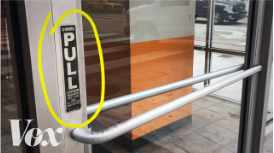
\includegraphics[scale = 0.7]{immagini/sign.png}
	\caption{La scritta pull è un significante, data l'affordance della porta di essere spinta o tirata.}
\end{figure}
\begin{figure}[!h]
	\centering
	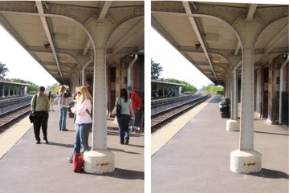
\includegraphics[scale = 0.7]{immagini/sign1.png}
	\caption{Le persone che aspettano il treno sono un esempio di significante sociale.}
\end{figure}

\section{Mapping}
\textbf{Mapping} è un termine tecnico, ripreso dalla matematica, che indica la relazione fra gli elementi di due insiemi.

Il concetto di mapping è di grande importanza nel progettare le interfacce e stabilire i significanti. La disposizione dei significanti può comunicare di più circa l'interfaccia e circa le sue funzionalità. Infatti quando il mapping usa una corrispondenza spaziale fra la collocazione dei comandi e quella dei dispositivi comandati, è facile capire come usarli.

Il modo migliore per applicare il mapping è quello \textbf{naturale}, perché è un'attività in cui il nostro cervello è molto bravo, i bambini imparano a fare mapping fin dai primi anni di vita. È da tenere presente che il concetto di \textbf{naturale} è ben diverso dal concetto di \textbf{universale}, poiché ci possono essere molti mapping che sembrano "naturali" ma sono specifici a una cerchia di culture.

\begin{figure}[!h]
	\centering
	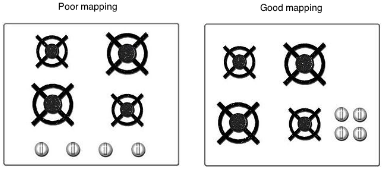
\includegraphics[scale = 0.7]{immagini/mapping.png}
	\caption{Mapping cattivo e mapping buono.}
\end{figure}

\pagebreak

\section{Feedback}
Il feedback è la comunicazione del risultato di un'azione, di una risposta dell'interfaccia verso l'utente.

Il feedback \textbf{deve essere immediato}, anche un ritardo di un decimo di secondo può essere troppo, se il ritardo è troppo lungo l'utente potrebbe rinunciare all'attività che stava compiendo con quel prodotto e passare ad altro o addirittura non riuscire a comprendere l'origine del feedback.

\textbf{Deve essere informativo}, non deve portare con se troppa informazione, ma deve assolvere al proprio obiettivo, deve far capire che un'azione è in corso o che è stato prodotto il risultato che ci aspettiamo. Un scarso feedback può essere peggio di nessun feedback, perché distrae, crea confusione e quindi frustrazione da parte dell'utente.

Altro fattore importante è \textbf{la semplicità}, ovvero un feedback non deve essere pedante: troppi annunci o segnali portano le persone ad ignorarli in modo da perdere anche quei feedback cruciali e importanti. Il feedback deve essere \textbf{essenziale} e mantenere l'ambiente calmo e tranquillo.

\section{Modello concettuale}
Un modello concettuale è una descrizione altamente semplificata delle funzionalità di un sistema; non deve essere completa o accurata ma utile. I file, le cartelle e le icone che vediamo sullo schermo del computer ci aiutano a creare un modello concettuale dei dati in memoria o delle applicazioni disponibili. In realtà il computer non contiene fascicoli o cartelle: esse sono solo concettualizzazioni ideate per facilitarne l'uso.

\textbf{I modelli semplificati sono preziosi e utili fintanto che le ipotesi che li supportano sono vere.}

Nel Cloud Storage Sync i file sembrano essere sul dispositivo, ma in molti casi il materiale è nel cloud. Il modello concettuale è quello di un archivio disponibile sui dispositivi degli utenti. Questo modello semplificato è utile per il normale utilizzo, ma se il collegamento dei servizi si interrompe, può nascere confusione: l'informazione è sempre presente sullo schermo, ma non possiamo più salvarla o recuperare altri dati, cosa inspiegabile in relazione al modello concettuale precedentemente citato.

Il modello concettuale è \textbf{come il designer vuole che l'utente percepisca il prodotto}; sarebbe l'ambizione di progettare e comprendere la UX.

Una volta che i progettisti hanno pensato e progettato il modello concettuale si implementa l'interfaccia, in modo che il modello concettuale venga veicolato all'utente tramite affordance, significanti e mapping presenti su essa.

Quando una persona si interfaccia con il sistema o il prodotto sviluppa un suo modello mentale. Un \textbf{modello mentale} è un modello concettuale nella mente dell'utente che rappresenta il modo in cui, secondo lui, funzionano le cose. Non solo persone diverse possono avere modelli mentali diversi dello stesso oggetto, ma la stessa persona può avere molteplici modelli, pertinenti ciascuno a un aspetto diverso del suo funzionamento, e persino contraddittori gli uni con gli altri.

\textbf{Più è grande la differenza tra il modello mentale e quello concettuale, più l'utente farà fatica ad usare il sistema.}

L'ideale è che l'utente apprenda un modello concettuale giusto \textbf{direttamente dal device che utilizza}, senza andare a leggere manuali o istruzioni o, peggio ancora, trasmessi da persona a persona. La comprensione di un dispositivo tramite passaparola porta all'effetto del "telefono senza fili": l'interpretazione cambia da persona a persona. Per questo vi è necessità che il modello concettuale trasmesso dal prodotto sia pressoché univoco con quello mentale che l'utente si è fatto.

In questo contesto vale l'affermazione \textit{less is more} secondo cui se una feature è difficile da veicolare allora è meglio non implementarla.

\section{Immagine di Sistema}
Le persone si creano di continuo modelli mentali di sé, degli altri, dell'ambiente degli oggetti con cui interagiscono: modelli concettuali formati attraverso l'esperienza, l'addestramento e l'istruzione.

Questi modelli ci servono da guida per realizzare i nostri scopi e comprendere il mondo in cui viviamo.

Come ci formiamo un modello concettuale adeguato dei dispositivi che utilizziamo? Non potendo parlare con il progettista, ci basiamo su tutta l'informazione accessibile: l'aspetto dell'apparecchio, cosa abbiamo imparato dall'uso di oggetti simili in passato, cosa ci dicono le pubblicità, i venditori, i pieghevoli illustrativi, il sito web e il libretto di istruzioni. \textbf{L'insieme di tutta questa informazione è l'immagine di sistema}.

\begin{figure}[!h]
	\centering
	\includegraphics[scale = 0.75]{"immagini/Immagine di Sistema"}
\end{figure}

Come illustrato nella figura, il progettista e l'utilizzatore finale del prodotto costituiscono i vertici scollegati di un triangolo. Un vertice del triangolo è occupato dal modello concettuale del progettista, \textbf{cioè dalla sua concezione del prodotto in questione}.

Una volta commercializzato, il prodotto si stacca dal progettista: lo vediamo isolato al secondo vertice del triangolo.

\textbf{L'immagine di sistema è tutto ciò che si percepisce dalla struttura fisica prodotta (completa di documentazione, istruzioni,significanti e ogni informazione accessibile dal sito web o dal servizio di assistenza clienti)}.

Il modello concettuale dell'utente deriva dall'immagine di sistema, mediante l'interazione con prodotto, letture, ricerca online e manuali. Il progettista si aspetta che il modello concettuale dell'utente coincida col suo, ma, non essendoci comunicazione diretta fra lui e l'utente, tutto il peso della comunicazione grava sull'immagine di sistema.

Questo spiega perché la comunicazione è un aspetto importante del buon design.\textbf{ Per quanto sia geniale il prodotto, se la gente non riesce ad usarlo l'accoglienza sarà cattiva}. Tocca al progettista fornire l'informazione adeguata a renderlo comprensibile e usabile. Quel che più conta è presentare un modello concettuale capace di guidare l'utente quando le cose non vanno come dovrebbero.

Un buon modello concettuale è la chiave per avere prodotti comprensibili, di facile uso e gradevole. La buona comunicazione è la chiave per ottenere buoni modelli concettuali.

\pagebreak


\chapter{Constraints, Discoverability e Feedback}
\begin{flushleft}
	\textit{In che modo si riesce a capire una cosa che non abbiamo mai visto prima?}
\end{flushleft}

Non c'è altro da fare che combinare l'informazione presente nel mondo esterno con quella che abbiamo in testa.

L'insieme di conoscenze che troviamo nel mondo comprende le affordance, i significanti visibili, le corrispondenze fra quelle parti degli oggetti che sembrano comandi o punti da manipolare, le azioni risultanti e i vincoli fisici, che limitano ciò che è possibile fare.

La conoscenza che abbiamo in mente comprende i modelli concettuali, i vincoli culturali, semantici e logici del comportamento, le analogie fra la situazione attuale ed esperienze precedenti.

\begin{figure}[!h]
	\centering
	\includegraphics[scale = 0.7]{"immagini/Modellino Lego"}
	\caption{Un modellino lego.}
\end{figure}

Prendiamo come esempio il modellino Lego presente in figura: ha 15 pezzi, solo alcuni specializzati, molti altri sono di grandezza e forma uguale ma di colori diversi. Ma combinando i vincoli fisici con quelli culturali, semantici e logici si riesce a costruire il modellino senza istruzioni, mettendo ogni pezzo nella sua giusta posizione.

Vincoli fisici limitano le parti che possono andare insieme, i vincoli culturali e semantici impongono restrizioni precise a tutti i pezzi restanti e se rimane fuori qualche pezzo l'incastro è dettato dalla logica.

\textbf{I vincoli sono indizi potenti}, che limitano l'insieme delle azioni possibili. L'uso intelligente dei vincoli in sede di design permette alle persone di decidere prontamente il giusto corso d'azione, anche in una situazione del tutto nuova.

\pagebreak

Possiamo categorizzare i vincoli in \textbf{quattro} classi:
\begin{itemize}
	\item \textbf{Vincoli fisici}: si affidano a proprietà del mondo fisico, senza alcun bisogno di istruzioni o di addestramento. Nell'esempio della motocicletta Lego ritroviamo questo vincolo nei pezzi che si incastrano solo in un determinato verso.
	\item \textbf{Vincoli culturali}: si affidano alle abitudini culturali, sociali, comportamentali che possono cambiare nel tempo. Con vincolo culturale si intendono anche le convenzioni. Nell'esempio della motocicletta Lego ritroviamo questo vincolo nel saper determinare la collocazione delle luci: bianco all'anteriore e rosso al posteriore.
	\item \textbf{Vincoli semantici}: si affidano al significato della situazione per circoscrivere l'insieme delle azioni possibili, si basano sulla conoscenza della situazione e del mondo. Nel caso della motocicletta, c'è un'unica collocazione sensata per il motociclista, deve stare seduto guardando in avanti.
	\item \textbf{Vincoli logici}: dettati dalla semplice e pura logica umana. Se avanzasse un un solo pezzo per assemblare la motocicletta, grazie alla logica sapremo dove collocarlo nella sua giusta posizione.
\end{itemize}

Un buon designer può sfruttare questi vincoli per veicolare l'utente verso un modello mentale del prodotto che si avvicini il più possibile al modello concettuale desiderato ed in tal modo garantirgli una UX gradevole.

\section{Vincoli e mapping}
Vincoli e mapping a volte si confondono tra di loro. Una serie di interruttori mappati in maniera opportuna danno un vincolo logico che permette all'utente di non sbagliare, si intuisce perfettamente cosa verrà azionato da quell'interruttore posto in quel determinato punto. \textbf{Mapping forti diventano quasi dei vincoli logici}.
L'assenza di vincoli e mapping genera, come detto più volte, frustrazione poiché crea una interfaccia poco chiara e difficile da comprendere.
\begin{figure}[!h]
	\centering
	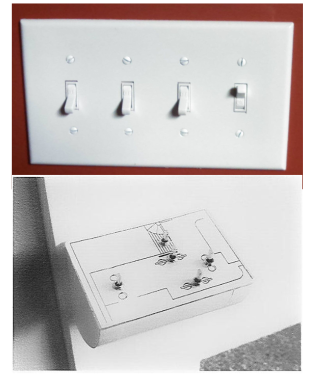
\includegraphics[scale=0.67]{immagini/Interruttori}
	\caption{Un interruttore per le luci di una stanza che imita la piantina del locale.}
\end{figure}

\pagebreak

\section{Funzioni Obbliganti}
\textbf{Le funzioni obbliganti sono una forma di vincolo fisico}: consistono di situazioni in cui le azioni sono vincolate in modo che un passaggio mancato impedisce di procedere al successivo.

Sono il caso estremo di vincoli per impedire un comportamento inappropriato.

Non tutte le situazioni permettono l'intervento di vincoli così forti, ma il principio generale si applica negli ambiti più diversi.

Esaminiamo tre di questi metodi per applicare funzioni obbliganti:
\begin{itemize}
	\item \textbf{Interlock}: obbliga a eseguire le operazioni nella sequenza dovuta. Usati soprattutto nell'ambito della sicurezza. \textbf{Per compiere un task si deve eseguire una serie di passi.}
	\item \textbf{Lock-in}: mantiene attiva una funzione impedendo che qualcuno la interrompa prematuramente. Usato molto in ambito informatico (e.g. ogni tentativo di uscita da un'applicazione senza salvare è prevenuto da un messaggio di allerta che chiede la conferma dell'intenzione). \textbf{Per finire un task si deve compiere un'azione.}
	\item \textbf{Lockout}: impedisce l'ingresso in uno spazio pericoloso o impedisce che succeda qualcosa. Può essere considerato l'opposto del lock-in. Un esempio di stampo informatico, sono gli alert "VM 18" dove dobbiamo dichiarare la maggiore età che si possono trovare su alcuni siti. \textbf{Per iniziare un task si deve compiere un'azione.}
\end{itemize}

\begin{figure}[!h]
	\centering
	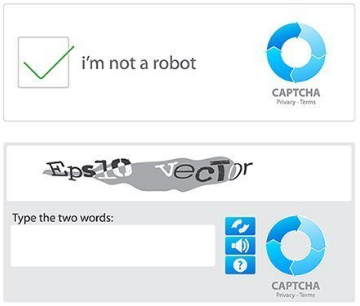
\includegraphics[scale=0.4]{immagini/cap.png}
	\caption{I captcha sono un esempio di interlocks.}
\end{figure}

\section{Activity-Centered Control}
Il mapping spaziale dei comandi non sempre è il più opportuno.

In molti casi è meglio avere interruttori diversi per attività diverse: \textbf{comandi centrati sulle attività}.

Quindi azionando un semplice comando si imposta una serie di oggetti per svolgere una determinata attività, senza comandarne uno per uno. In molti auditorium ci sono interruttori con indicazioni "video", "computer", "piena luce", "lezione" che impostano il microfono, le luci della sala, il proiettore e quant'altro, nel miglior modo per svolgere l'attività selezionata.

Questo schema è eccellente in teoria, ma nella pratica è difficile da realizzare bene, soprattutto è necessario valutare gli imprevisti e le possibili risoluzioni.

Il metodo è giusto, purché la gamma di attività sia scelta in modo da rispondere alle situazioni reali. Ma anche in quel caso saranno pur necessari dei comandi manuali, perché si presenteranno sempre esigenze inattese, che richiederanno una regolazione particolare dei dispositivi.


\chapter{How do people do things}
\begin{flushleft}
	\textit{
		È facile imparare alcune azioni elementari per far funzionare un dispositivo tecnico. Ma cosa succede se le cose non vanno come dovrebbero? Come può l'utente accorgersene, e scoprire cosa fare? }
\end{flushleft}

Per chiarire meglio tutto questo è bene soffermarsi sulla psicologia umana e su un semplice modello concettuale dei modi in cui si sceglie e si valutano le nostre azioni. Da qui si passerà a esaminare il ruolo della cognizione e delle emozioni: piacere quando le cose funzionano senza intoppi, frustrazione quando le nostre aspettative iniziali sono bloccate.

\section{I Golfi dell'Esecuzione e della Valutazione}
Quando usiamo un oggetto, ci troviamo davanti due golfi: il \textbf{golfo dell'esecuzione}, nel quale cerchiamo di indovinare come funziona e cosa fare, e il \textbf{golfo della valutazione}, in cui si tratta di capire cosa succede. Il compito del progettista è aiutare le persone a superare i due golfi e renderli il meno profondi possibili.

\begin{figure}[!h]
	\centering
	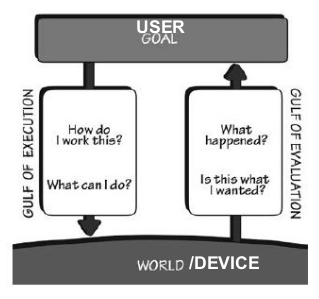
\includegraphics[scale=0.7]{immagini/Golfi}
	\caption{Golfo dell'esecuzione e golfo della valutazione.}
\end{figure}

Il \textbf{golfo della valutazione} corrisponde allo sforzo necessario per interpretare lo stato fisico del dispositivo e capire fino a che punto sono realizzate aspettative e intenzioni. Il Golfo è stretto quando il dispositivo fornisce informazioni sul proprio stato, in una forma facile da cogliere e interpretare, e corrispondente all'idea che abbiamo del suo funzionamento.

\pagebreak

\textit{\begin{flushleft}
		Quali sono gli elementi progettuali più importanti per superare il golfo della valutazione?
	\end{flushleft}}
Il feedback e un modello concettuale adeguato.

\begin{flushleft}
	\textit{Quali sono gli elementi progettuali più importanti per superare il golfo dell' esecuzione?}
\end{flushleft}
Significanti, constraints, mapping e un modello concettuale.

Entrambi i golfi sono presenti in molti apparati. Si incontrano spesso difficoltà, ma ogni volta vengono liquidate accusando se stessi. Di fronte a queste cose che ci si aspetterebbe di saper usare, si conclude semplicemente con \textit{"sono stupido"}. Oppure, con dispositivi dall'aspetto più complicato, semplicemente ci si arrende, pensando di essere incapaci di utilizzarli. Queste spiegazioni sono entrambe sbagliate. \textbf{Le difficoltà hanno origine nel desing, non nell'utente}.

\section{I sette stadi dell'azione}
Un'azione implica due fasi: \textbf{eseguirla e valutarne gli effetti}, \textbf{fare e interpretare}. Sia l'esecuzione che la valutazione richiedono che si capisca come funziona una cosa e quali risultati produce. Entrambe le fasi influiscono sul nostro stato emotivo.

Le azioni specifiche fanno da ponte fra ciò che vorremmo veder realizzato e tutte le possibili azioni fisiche per arrivarci. Una volta specificato quali azioni compiere, dobbiamo effettuarle concretamente: questo è lo \textbf{stadio dell'esecuzione}. \textbf{Dallo scopo discendono i tre stadi dell'esecuzione: pianificare, specificare ed eseguire.}

\textbf{La valutazione si articola anch'essa in tre stadi: percepire, interpretazione, confrontare.}

Ecco così che abbiamo i \textbf{sette stadi dell'azione}: uno per lo scopo, tre per l'esecuzione e tre per la valutazione.
\begin{itemize}
	\item \textbf{Scopo}: definire l'obiettivo.
	\item \textbf{Progettare}: l'azione da eseguire.
	\item \textbf{Specificare}: una sequenza d'azione.
	\item \textbf{Eseguire}: la sequenza specificata.
	\item \textbf{Percepire}: lo stato del mondo.
	\item \textbf{Interpretare}: la percezione.
	\item \textbf{Confrontare}: il risultato con lo scopo.
\end{itemize}
\begin{center}
	\includegraphics[width=0.5\linewidth]{"immagini/Sette stadi"}
\end{center}
La maggior parte delle azioni non richiede tutti i sette stadi in sequenza, ma quasi nessuna attività si risolve in un'azione singola.

Di solito intervengono numerose sequenze e l'intera attività può durare ore o giorni. Ci sono molteplici circuiti di feedback, con cui i risultati di un'attività sono usati per indirizzare l'utente verso altre, in cui uno scopo genera scopi accessori, un progetto sotto-progetti. Ci sono attività in cui lo scopo originario è dimenticato, scartato o riformulato.

I sette stadi offrono uno schema per sviluppare nuovi prodotti o servizi. I golfi dell'esecuzione e della valutazione sono i punti più ovvi da cui partire, poiché entrambi offrono l'occasione di migliorare il prodotto. Tutto sta nello sviluppare capacità di osservazione per scoprirli.

\section{Tre livelli di Processing}
Gli stadi dell'azione possono essere associati con tre livelli di processing mentale: viscerale, comportamentale e riflessivo.

\begin{itemize}
	\item \textbf{Livello viscerale}: è il livello più elementare che ci permette di rispondere prontamente in maniera subconscia, senza consapevolezza o controllo cosciente.
	\item \textbf{Livello comportamentale}: è la sede delle abilità apprese, attivate da situazioni che corrispondono al modello pertinente. In sede di design, il livello comportamentale è guidato dalle aspettative durante l'esecuzione e guidato dalle emozioni durante l'attesa di conferme di tali aspettative. Decide in che modo si compie un determinato task e in che modo si interpreta un determinato feedback.
	\item \textbf{Livello riflessivo}: è quello della cognizione conscia, è quindi a questo livello che si sviluppa la comprensione profonda e hanno luogo il ragionamento e i processi decisionali. Qui fanno capo i livelli più alti di emotività: è qui che avviene la soddisfazione e l'orgoglio, ma anche la frustrazione e il senso di colpa.
\end{itemize}

\begin{figure}[!h]
	\centering
	\includegraphics[scale=1]{"immagini/Livelli di Processing"}
\end{figure}

\textbf{Per il progettista il livello riflessivo è forse il più importante dei tre}. La riflessione è conscia e le emozioni che si producono a questo livello sono le più durature: quelle che attribuiscono responsabilità agli agenti casuali, come colpa, vergogna e orgoglio.

Le risposte riflessive sono anche parte integrante del ricordo degli eventi, che dura assai più a lungo dell'esperienza immediata o del periodo d'uso, che sono invece ambiti del livello viscerale e comportamentale.

È la riflessione che ci induce a consigliare un prodotto, a raccomandare l'uso o magari a sconsigliarlo.

I tre livelli di elaborazione contribuiscono tutti insieme a determinare il nostro stato emotivo e cognitivo. Funzioni riflessive di alto livello possono mettere in moto le emozioni più elementari, così come queste possono stimolare attività cognitive di tipo riflessivo.

\section{I sette Principi Fondamentali della Progettazione}
Il modello in sette stadi del ciclo d'azione può essere un prezioso sussidio per il design, in quanto suggerisce una lista di domande fondamentali. In generale, ogni stadio dell'azione richiede specifiche strategie progettuali, e, viceversa, presenta occasioni tutte sue di disastro.

Derivano quindi sette domande, a cui dovrebbe poter rispondere chiunque stia usando un determinato prodotto.

\begin{itemize}
	\item \textbf{Cosa voglio ottenere?}
	\item \textbf{Quali sono le sequenze d'azione alternative?}
	\item \textbf{Quale azione posso fare ora?}
	\item \textbf{Come faccio questa azione?}
	\item \textbf{Cosa è successo?}
	\item \textbf{Cosa significa?}
	\item \textbf{Va bene? Ho realizzato il mio scopo?}
\end{itemize}

\begin{figure}[!h]
	\centering
	\includegraphics[scale=0.55]{"immagini/Sette Domande"}
\end{figure}

\pagebreak

Il progettista ha la responsabilità di garantire che a ogni stadio dell'azione il prodotto fornisca l'informazione necessaria per la risposta.

L'informazione che serve a rispondere alle domande sull'esecuzione è il \textbf{feedforward}.

L'informazione che aiuta a capire quello che è successo è il \textbf{feedback}.

Il \textbf{feedforward} si realizza mediante l'uso opportuno di significanti, vincoli e mapping, anche il modello concettuale ha un ruolo importante. Il \textbf{feedback} è dato dall'informazione esplicita circa l'impatto dell'azione eseguita e anche qui una parte importante è svolta dal modello concettuale.

Sia il \textbf{feedback}, che il \textbf{feedforward} devono presentarsi in una forma facilmente interpretabile da chi utilizza il sistema. La presentazione deve corrispondere alla visione che le persone hanno dello scopo che vogliono realizzare e alle loro aspettative. L'informazione deve essere congruente con le esigenze umane.

Dalle risposte relative ai sette stadi dell'azione si ricavano sette principi fondamentali del design:

\begin{itemize}
	\item \textbf{Visibilità}: è possibile scoprire immediatamente quali azioni sono possibili e qual è lo stato attuale del dispositivo.
	\item \textbf{Feedback}: c'è un'informazione completa e continua riguardo ai risultati delle azioni e allo stato attuale del prodotto o del servizio. Dopo aver eseguito un'azione, è facile determinare il nuovo stato.
	\item \textbf{Modello Concettuale}: il design fornisce tutta l'informazione necessaria per creare un buon modello concettuale del sistema, che favorisca la comprensione e la sensazione di controllo. Il modello concettuale potenzia sia la visibilità, sia la valutazione dei risultati.
	\item \textbf{Affordance}: affordance corrette sono fatte apposta per rendere possibili le azioni desiderate.
	\item \textbf{Significanti}: un uso efficace dei significanti assicura la visibilità e un feedback efficiente e intellegibile.
	\item \textbf{Mapping}: la relazione  fra i comandi e le rispettive azioni obbedisce ai principi del buon mapping, sostenuto, per quanto possibile, dalla disposizione spaziale e dalla contiguità temporale.
	\item \textbf{Vincoli}: fornire vincoli fisici, logici, semantici e culturali guidando l'azione e facilitandone l'interpretazione.
\end{itemize}
Questi sette principi sono mappati uno a uno sugli stadi d'azione dell'utente.

È bene concludere con una nota la parte dedicata a strumenti, metodi ed elementi per il design dello human-computer interaction: per molte attività quotidiane , gli obiettivi e le interazioni non sono ben definiti, \textbf{sono più di tipo opportunistico che pianificato}.

Le azioni opportunistiche sono quelle in cui il comportamento scaturito dalle circostanze prevale sulla pianificazione. Gli utenti in questi casi agiscono in maniera non controllata e quindi non prevedibile.

È difficile fare buon design per queste situazioni, anche attenendosi a tutti i principi esposti fino ad ora: l'utente che agisce in maniera opportunistica romperà questi schemi.

\pagebreak

\section{Disruptive Innovation}
\begin{flushleft}
	\textit{“People don’t want to buy a quarter-inch drill. They want a quarter-inch hole!”}
\end{flushleft}
La maggior parte dell'innovazione è fatta come miglioramento incrementale di prodotti già esistenti. La \textbf{disruptive innovation} riguarda l'innovazione non lineare, consiste in un completo salto di binario. Vuole introdurre idee radicali che portano a progettare nuove categorie di prodotto nel mercato.

\begin{figure}[!h]
	\centering
	\includegraphics[scale=0.8]{"immagini/Disruptive Innovation"}
\end{figure}

Ciò è effettuato riconsiderando l'obbiettivo tramite un procedimento chiamato \textbf{root cause analysis}, che può essere decomposto in quattro fasi.

La \textbf{root cause analysis} è quindi fatta:

\begin{enumerate}
	\item Descrivendo chiaramente il problema.
	\item Tracciando il flusso degli eventi che ha fatto in modo che da una situazione di normalità emergesse un problema.
	\item Distinguendo le cause principali dalle cause secondarie.
	\item Tracciando un grafico che descrive le relazioni tra le cause principali e il problema.
\end{enumerate}







\end{document}